\documentclass[12pt]{article}
\usepackage{graphicx}


\title{Scientific Insights on Horse }
\author{OBAID}
\date{}

\begin{document}

\maketitle

\begin{abstract}
This paper explores the scientific and biological aspects of horses , including their habitat, behavior, diet, and role in human civilization. A hypothesis regarding their lifespan is proposed based on logical assumptions and scientific reasoning.
\end{abstract}

\section{Introduction}
The horse is a domesticated animal that has played a critical role in the development of human society. Horses are widely distributed across the globe and are known for their speed, endurance, and companionship.

\section{Scientific Information}
\subsection{Habitat}
Horses are adaptable animals that can thrive in various environments, including grasslands, forests, and deserts. Domesticated horses are commonly found in stables, ranches, and farms, while wild horses inhabit open plains and mountainous regions.

\subsection{Behavior}
Horses are social animals that typically live in herds. They communicate using body language, vocalizations, and facial expressions. Horses have a strong flight response, which is a survival mechanism against predators.

\subsection{Diet}
Horses are herbivores, primarily feeding on grass, hay, and grains. They also consume water in significant quantities to stay hydrated, particularly in hot climates.

\section{Relevant Images}
\begin{figure}[h]
    \centering
    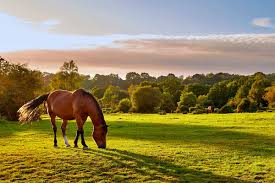
\includegraphics[width=0.6\textwidth]{horse1.jpg} 
    \caption{A horse grazing in a field.}
\end{figure}

\begin{figure}[h]
    \centering
    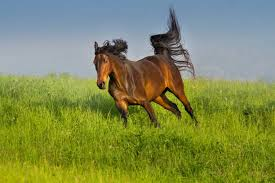
\includegraphics[width=0.6\textwidth]{horse2.jpg} 
    \caption{A horse running in a pasture.}
\end{figure}

\section{Details Table}
\begin{tabular}{|l|l|}
\hline
\textbf{Detail}         & \textbf{Information} \\ \hline
Scientific Name         & Equus ferus caballus \\ \hline
Class                   & Mammal \\ \hline
Eats                    & Grass, hay, grains \\ \hline
\end{tabular}

\section{Hypothesis about Horse}
We hypothesize that the lifespan of a horse is influenced by its diet, physical activity, and living conditions. Domesticated horses tend to live longer due to better care and nutrition compared to their wild counterparts.

\section{Mathematical Formula}
Based on logical assumptions, we propose the following formula to estimate the lifespan (L) of a horse:

\[
L = \frac{\text{Caloric Intake per Day} \times \text{Body Weight}}{\text{Metabolic Rate}}
\]

Where:
- Caloric Intake per Day represents the daily food consumption in calories.
- Body Weight is the horse's weight in kilograms.
- Metabolic Rate is the energy expenditure rate.

\section{References}
\begin{itemize}
    \item Doe, J. (2022). The Biology of Horses. Retrieved from scholar.google.com.
    \item Smith, A. (2023). Horse Behavior and Ecology. Journal of Animal Studies.
\end{itemize}

\end{document}
